


% Header, overrides base

    % Make sure that the sphinx doc style knows who it inherits from.
    \def\sphinxdocclass{article}

    % Declare the document class
    \documentclass[letterpaper,10pt,english]{/usr/local/lib/python2.7/dist-packages/sphinx/texinputs/sphinxhowto}

    % Imports
    \usepackage[utf8]{inputenc}
    \DeclareUnicodeCharacter{00A0}{\\nobreakspace}
    \usepackage[T1]{fontenc}
    \usepackage{babel}
    \usepackage{times}
    \usepackage{import}
    \usepackage[Bjarne]{/usr/local/lib/python2.7/dist-packages/sphinx/texinputs/fncychap}
    \usepackage{longtable}
    \usepackage{/usr/local/lib/python2.7/dist-packages/sphinx/texinputs/sphinx}
    \usepackage{multirow}

    \usepackage{amsmath}
    \usepackage{amssymb}
    \usepackage{ucs}
    \usepackage{enumerate}

    % Used to make the Input/Output rules follow around the contents.
    \usepackage{needspace}

    % Pygments requirements
    \usepackage{fancyvrb}
    \usepackage{color}
    % ansi colors additions
    \definecolor{darkgreen}{rgb}{.12,.54,.11}
    \definecolor{lightgray}{gray}{.95}
    \definecolor{brown}{rgb}{0.54,0.27,0.07}
    \definecolor{purple}{rgb}{0.5,0.0,0.5}
    \definecolor{darkgray}{gray}{0.25}
    \definecolor{lightred}{rgb}{1.0,0.39,0.28}
    \definecolor{lightgreen}{rgb}{0.48,0.99,0.0}
    \definecolor{lightblue}{rgb}{0.53,0.81,0.92}
    \definecolor{lightpurple}{rgb}{0.87,0.63,0.87}
    \definecolor{lightcyan}{rgb}{0.5,1.0,0.83}

    % Needed to box output/input
    \usepackage{tikz}
        \usetikzlibrary{calc,arrows,shadows}
    \usepackage[framemethod=tikz]{mdframed}

    \usepackage{alltt}

    % Used to load and display graphics
    \usepackage{graphicx}
    \graphicspath{ {figs/} }
    \usepackage[Export]{adjustbox} % To resize

    % used so that images for notebooks which have spaces in the name can still be included
    \usepackage{grffile}


    % For formatting output while also word wrapping.
    \usepackage{listings}
    \lstset{breaklines=true}
    \lstset{basicstyle=\small\ttfamily}
    \def\smaller{\fontsize{9.5pt}{9.5pt}\selectfont}

    %Pygments definitions
    
\makeatletter
\def\PY@reset{\let\PY@it=\relax \let\PY@bf=\relax%
    \let\PY@ul=\relax \let\PY@tc=\relax%
    \let\PY@bc=\relax \let\PY@ff=\relax}
\def\PY@tok#1{\csname PY@tok@#1\endcsname}
\def\PY@toks#1+{\ifx\relax#1\empty\else%
    \PY@tok{#1}\expandafter\PY@toks\fi}
\def\PY@do#1{\PY@bc{\PY@tc{\PY@ul{%
    \PY@it{\PY@bf{\PY@ff{#1}}}}}}}
\def\PY#1#2{\PY@reset\PY@toks#1+\relax+\PY@do{#2}}

\expandafter\def\csname PY@tok@gd\endcsname{\def\PY@tc##1{\textcolor[rgb]{0.63,0.00,0.00}{##1}}}
\expandafter\def\csname PY@tok@gu\endcsname{\let\PY@bf=\textbf\def\PY@tc##1{\textcolor[rgb]{0.50,0.00,0.50}{##1}}}
\expandafter\def\csname PY@tok@gt\endcsname{\def\PY@tc##1{\textcolor[rgb]{0.00,0.27,0.87}{##1}}}
\expandafter\def\csname PY@tok@gs\endcsname{\let\PY@bf=\textbf}
\expandafter\def\csname PY@tok@gr\endcsname{\def\PY@tc##1{\textcolor[rgb]{1.00,0.00,0.00}{##1}}}
\expandafter\def\csname PY@tok@cm\endcsname{\let\PY@it=\textit\def\PY@tc##1{\textcolor[rgb]{0.25,0.50,0.50}{##1}}}
\expandafter\def\csname PY@tok@vg\endcsname{\def\PY@tc##1{\textcolor[rgb]{0.10,0.09,0.49}{##1}}}
\expandafter\def\csname PY@tok@m\endcsname{\def\PY@tc##1{\textcolor[rgb]{0.40,0.40,0.40}{##1}}}
\expandafter\def\csname PY@tok@mh\endcsname{\def\PY@tc##1{\textcolor[rgb]{0.40,0.40,0.40}{##1}}}
\expandafter\def\csname PY@tok@go\endcsname{\def\PY@tc##1{\textcolor[rgb]{0.53,0.53,0.53}{##1}}}
\expandafter\def\csname PY@tok@ge\endcsname{\let\PY@it=\textit}
\expandafter\def\csname PY@tok@vc\endcsname{\def\PY@tc##1{\textcolor[rgb]{0.10,0.09,0.49}{##1}}}
\expandafter\def\csname PY@tok@il\endcsname{\def\PY@tc##1{\textcolor[rgb]{0.40,0.40,0.40}{##1}}}
\expandafter\def\csname PY@tok@cs\endcsname{\let\PY@it=\textit\def\PY@tc##1{\textcolor[rgb]{0.25,0.50,0.50}{##1}}}
\expandafter\def\csname PY@tok@cp\endcsname{\def\PY@tc##1{\textcolor[rgb]{0.74,0.48,0.00}{##1}}}
\expandafter\def\csname PY@tok@gi\endcsname{\def\PY@tc##1{\textcolor[rgb]{0.00,0.63,0.00}{##1}}}
\expandafter\def\csname PY@tok@gh\endcsname{\let\PY@bf=\textbf\def\PY@tc##1{\textcolor[rgb]{0.00,0.00,0.50}{##1}}}
\expandafter\def\csname PY@tok@ni\endcsname{\let\PY@bf=\textbf\def\PY@tc##1{\textcolor[rgb]{0.60,0.60,0.60}{##1}}}
\expandafter\def\csname PY@tok@nl\endcsname{\def\PY@tc##1{\textcolor[rgb]{0.63,0.63,0.00}{##1}}}
\expandafter\def\csname PY@tok@nn\endcsname{\let\PY@bf=\textbf\def\PY@tc##1{\textcolor[rgb]{0.00,0.00,1.00}{##1}}}
\expandafter\def\csname PY@tok@no\endcsname{\def\PY@tc##1{\textcolor[rgb]{0.53,0.00,0.00}{##1}}}
\expandafter\def\csname PY@tok@na\endcsname{\def\PY@tc##1{\textcolor[rgb]{0.49,0.56,0.16}{##1}}}
\expandafter\def\csname PY@tok@nb\endcsname{\def\PY@tc##1{\textcolor[rgb]{0.00,0.50,0.00}{##1}}}
\expandafter\def\csname PY@tok@nc\endcsname{\let\PY@bf=\textbf\def\PY@tc##1{\textcolor[rgb]{0.00,0.00,1.00}{##1}}}
\expandafter\def\csname PY@tok@nd\endcsname{\def\PY@tc##1{\textcolor[rgb]{0.67,0.13,1.00}{##1}}}
\expandafter\def\csname PY@tok@ne\endcsname{\let\PY@bf=\textbf\def\PY@tc##1{\textcolor[rgb]{0.82,0.25,0.23}{##1}}}
\expandafter\def\csname PY@tok@nf\endcsname{\def\PY@tc##1{\textcolor[rgb]{0.00,0.00,1.00}{##1}}}
\expandafter\def\csname PY@tok@si\endcsname{\let\PY@bf=\textbf\def\PY@tc##1{\textcolor[rgb]{0.73,0.40,0.53}{##1}}}
\expandafter\def\csname PY@tok@s2\endcsname{\def\PY@tc##1{\textcolor[rgb]{0.73,0.13,0.13}{##1}}}
\expandafter\def\csname PY@tok@vi\endcsname{\def\PY@tc##1{\textcolor[rgb]{0.10,0.09,0.49}{##1}}}
\expandafter\def\csname PY@tok@nt\endcsname{\let\PY@bf=\textbf\def\PY@tc##1{\textcolor[rgb]{0.00,0.50,0.00}{##1}}}
\expandafter\def\csname PY@tok@nv\endcsname{\def\PY@tc##1{\textcolor[rgb]{0.10,0.09,0.49}{##1}}}
\expandafter\def\csname PY@tok@s1\endcsname{\def\PY@tc##1{\textcolor[rgb]{0.73,0.13,0.13}{##1}}}
\expandafter\def\csname PY@tok@sh\endcsname{\def\PY@tc##1{\textcolor[rgb]{0.73,0.13,0.13}{##1}}}
\expandafter\def\csname PY@tok@sc\endcsname{\def\PY@tc##1{\textcolor[rgb]{0.73,0.13,0.13}{##1}}}
\expandafter\def\csname PY@tok@sx\endcsname{\def\PY@tc##1{\textcolor[rgb]{0.00,0.50,0.00}{##1}}}
\expandafter\def\csname PY@tok@bp\endcsname{\def\PY@tc##1{\textcolor[rgb]{0.00,0.50,0.00}{##1}}}
\expandafter\def\csname PY@tok@c1\endcsname{\let\PY@it=\textit\def\PY@tc##1{\textcolor[rgb]{0.25,0.50,0.50}{##1}}}
\expandafter\def\csname PY@tok@kc\endcsname{\let\PY@bf=\textbf\def\PY@tc##1{\textcolor[rgb]{0.00,0.50,0.00}{##1}}}
\expandafter\def\csname PY@tok@c\endcsname{\let\PY@it=\textit\def\PY@tc##1{\textcolor[rgb]{0.25,0.50,0.50}{##1}}}
\expandafter\def\csname PY@tok@mf\endcsname{\def\PY@tc##1{\textcolor[rgb]{0.40,0.40,0.40}{##1}}}
\expandafter\def\csname PY@tok@err\endcsname{\def\PY@bc##1{\setlength{\fboxsep}{0pt}\fcolorbox[rgb]{1.00,0.00,0.00}{1,1,1}{\strut ##1}}}
\expandafter\def\csname PY@tok@kd\endcsname{\let\PY@bf=\textbf\def\PY@tc##1{\textcolor[rgb]{0.00,0.50,0.00}{##1}}}
\expandafter\def\csname PY@tok@ss\endcsname{\def\PY@tc##1{\textcolor[rgb]{0.10,0.09,0.49}{##1}}}
\expandafter\def\csname PY@tok@sr\endcsname{\def\PY@tc##1{\textcolor[rgb]{0.73,0.40,0.53}{##1}}}
\expandafter\def\csname PY@tok@mo\endcsname{\def\PY@tc##1{\textcolor[rgb]{0.40,0.40,0.40}{##1}}}
\expandafter\def\csname PY@tok@kn\endcsname{\let\PY@bf=\textbf\def\PY@tc##1{\textcolor[rgb]{0.00,0.50,0.00}{##1}}}
\expandafter\def\csname PY@tok@mi\endcsname{\def\PY@tc##1{\textcolor[rgb]{0.40,0.40,0.40}{##1}}}
\expandafter\def\csname PY@tok@gp\endcsname{\let\PY@bf=\textbf\def\PY@tc##1{\textcolor[rgb]{0.00,0.00,0.50}{##1}}}
\expandafter\def\csname PY@tok@o\endcsname{\def\PY@tc##1{\textcolor[rgb]{0.40,0.40,0.40}{##1}}}
\expandafter\def\csname PY@tok@kr\endcsname{\let\PY@bf=\textbf\def\PY@tc##1{\textcolor[rgb]{0.00,0.50,0.00}{##1}}}
\expandafter\def\csname PY@tok@s\endcsname{\def\PY@tc##1{\textcolor[rgb]{0.73,0.13,0.13}{##1}}}
\expandafter\def\csname PY@tok@kp\endcsname{\def\PY@tc##1{\textcolor[rgb]{0.00,0.50,0.00}{##1}}}
\expandafter\def\csname PY@tok@w\endcsname{\def\PY@tc##1{\textcolor[rgb]{0.73,0.73,0.73}{##1}}}
\expandafter\def\csname PY@tok@kt\endcsname{\def\PY@tc##1{\textcolor[rgb]{0.69,0.00,0.25}{##1}}}
\expandafter\def\csname PY@tok@ow\endcsname{\let\PY@bf=\textbf\def\PY@tc##1{\textcolor[rgb]{0.67,0.13,1.00}{##1}}}
\expandafter\def\csname PY@tok@sb\endcsname{\def\PY@tc##1{\textcolor[rgb]{0.73,0.13,0.13}{##1}}}
\expandafter\def\csname PY@tok@k\endcsname{\let\PY@bf=\textbf\def\PY@tc##1{\textcolor[rgb]{0.00,0.50,0.00}{##1}}}
\expandafter\def\csname PY@tok@se\endcsname{\let\PY@bf=\textbf\def\PY@tc##1{\textcolor[rgb]{0.73,0.40,0.13}{##1}}}
\expandafter\def\csname PY@tok@sd\endcsname{\let\PY@it=\textit\def\PY@tc##1{\textcolor[rgb]{0.73,0.13,0.13}{##1}}}

\def\PYZbs{\char`\\}
\def\PYZus{\char`\_}
\def\PYZob{\char`\{}
\def\PYZcb{\char`\}}
\def\PYZca{\char`\^}
\def\PYZam{\char`\&}
\def\PYZlt{\char`\<}
\def\PYZgt{\char`\>}
\def\PYZsh{\char`\#}
\def\PYZpc{\char`\%}
\def\PYZdl{\char`\$}
\def\PYZhy{\char`\-}
\def\PYZsq{\char`\'}
\def\PYZdq{\char`\"}
\def\PYZti{\char`\~}
% for compatibility with earlier versions
\def\PYZat{@}
\def\PYZlb{[}
\def\PYZrb{]}
\makeatother


    %Set pygments styles if needed...
    
        \definecolor{nbframe-border}{rgb}{0.867,0.867,0.867}
        \definecolor{nbframe-bg}{rgb}{0.969,0.969,0.969}
        \definecolor{nbframe-in-prompt}{rgb}{0.0,0.0,0.502}
        \definecolor{nbframe-out-prompt}{rgb}{0.545,0.0,0.0}

        \newenvironment{ColorVerbatim}
        {\begin{mdframed}[%
            roundcorner=1.0pt, %
            backgroundcolor=nbframe-bg, %
            userdefinedwidth=1\linewidth, %
            leftmargin=0.1\linewidth, %
            innerleftmargin=0pt, %
            innerrightmargin=0pt, %
            linecolor=nbframe-border, %
            linewidth=1pt, %
            usetwoside=false, %
            everyline=true, %
            innerlinewidth=3pt, %
            innerlinecolor=nbframe-bg, %
            middlelinewidth=1pt, %
            middlelinecolor=nbframe-bg, %
            outerlinewidth=0.5pt, %
            outerlinecolor=nbframe-border, %
            needspace=0pt
        ]}
        {\end{mdframed}}
        
        \newenvironment{InvisibleVerbatim}
        {\begin{mdframed}[leftmargin=0.1\linewidth,innerleftmargin=3pt,innerrightmargin=3pt, userdefinedwidth=1\linewidth, linewidth=0pt, linecolor=white, usetwoside=false]}
        {\end{mdframed}}

        \renewenvironment{Verbatim}[1][\unskip]
        {\begin{alltt}\smaller}
        {\end{alltt}}
    

    % Help prevent overflowing lines due to urls and other hard-to-break 
    % entities.  This doesn't catch everything...
    \sloppy

    % Document level variables
    \title{Semilatice}
    \date{October 28, 2014}
    \release{}
    \author{Adrian Vrabie}
    \renewcommand{\releasename}{}

    % TODO: Add option for the user to specify a logo for his/her export.
    \newcommand{\sphinxlogo}{}

    % Make the index page of the document.
    \makeindex

    % Import sphinx document type specifics.
     


% Body

    % Start of the document
    \begin{document}

        
            \maketitle
        

        


        
        \section{Generalizarea Noțiunii de Latice:
Semilatice}\label{generalizarea-noux21biunii-de-latice-semilatice}

student: Adrian Vrabie

    % Make sure that atleast 4 lines are below the HR
    \needspace{4\baselineskip}

    
        \vspace{6pt}
        \makebox[0.1\linewidth]{\smaller\hfill\tt\color{nbframe-in-prompt}In\hspace{4pt}{[}1{]}:\hspace{4pt}}\\*
        \vspace{-2.65\baselineskip}
        \begin{ColorVerbatim}
            \vspace{-0.7\baselineskip}
            \begin{Verbatim}[commandchars=\\\{\}]
\PY{k+kn}{from} \PY{n+nn}{IPython.display} \PY{k+kn}{import} \PY{n}{YouTubeVideo}
\PY{k+kn}{from} \PY{n+nn}{IPython} \PY{k+kn}{import} \PY{n}{display}
\PY{k+kn}{from} \PY{n+nn}{IPython.display} \PY{k+kn}{import} \PY{n}{FileLink}\PY{p}{,} \PY{n}{FileLinks} \PY{c}{\PYZsh{} allows }
\end{Verbatim}

            
                \vspace{-0.2\baselineskip}
            
        \end{ColorVerbatim}
    
\subsection{Introducere}\label{introducere}

Pentru a înțelege laticele, avem nevoie de noțiunea unui set.
$A = \{"Bananna", "Apple", "Melon", "Kiwi", "Mango" \}$ este un set
arbitrar format din 5 elemente, însă nimic nu putem spune dacă acestă
mulțime este parțial ordonată.\subsection{Relație Binară}\label{relaux21bie-binarux103}

Ce este o relație binară ``$\preceq$'' sau se mai notează cu ``$*$'' ?

\begin{quote}
O relație binară $(*)$ în mulțimea $S$ este o funție (mapping) din
$S\times S \mapsto S$
\end{quote}

Sursa: \href{https://www.youtube.com/watch?v=gXxugQrrEgU}{Youtube Video}

    % Make sure that atleast 4 lines are below the HR
    \needspace{4\baselineskip}

    
        \vspace{6pt}
        \makebox[0.1\linewidth]{\smaller\hfill\tt\color{nbframe-in-prompt}In\hspace{4pt}{[}2{]}:\hspace{4pt}}\\*
        \vspace{-2.65\baselineskip}
        \begin{ColorVerbatim}
            \vspace{-0.7\baselineskip}
            \begin{Verbatim}[commandchars=\\\{\}]
\PY{n}{YouTubeVideo}\PY{p}{(}\PY{l+s}{\PYZsq{}}\PY{l+s}{gXxugQrrEgU?t=1m49s}\PY{l+s}{\PYZsq{}}\PY{p}{)}
\end{Verbatim}

            
                \vspace{-0.2\baselineskip}
            
        \end{ColorVerbatim}
    

    

        % If the first block is an image, minipage the image.  Else
        % request a certain amount of space for the input text.
        \needspace{4\baselineskip}
        
        

            % Add document contents.
            
                \makebox[0.1\linewidth]{\smaller\hfill\tt\color{nbframe-out-prompt}Out\hspace{4pt}{[}2{]}:\hspace{4pt}}\\*
                \vspace{-2.55\baselineskip}\begin{InvisibleVerbatim}
                \vspace{-0.5\baselineskip}
\begin{alltt}<IPython.lib.display.YouTubeVideo at 0x7febbce14710>\end{alltt}

            \end{InvisibleVerbatim}
            
        
    
\subsubsection{Ce este o mulțime Parțial
Ordonată?}\label{ce-este-o-mulux21bime-parux21bial-ordonatux103}Source:
\href{http://en.wikipedia.org/wiki/Partially_ordered_set}{Wikipedia}
\textgreater{}In mathematics, especially order theory, a partially
ordered set (or poset) formalizes and generalizes the intuitive concept
of an ordering, sequencing, or arrangement of the elements of a set. A
poset consists of a set together with a binary relation that indicates
that, for certain pairs of elements in the set, one of the elements
precedes the other. Such a relation is called a partial order to reflect
the fact that not every pair of elements need be related: for some
pairs, it may be that neither element precedes the other in the poset.
Thus, partial orders generalize the more familiar total orders, in which
every pair is related.Traducere: \textgreater{}O mulțime parțial ordonată (sau se mai numește
și \textbf{un set parțial ordonat} (sau \textbf{poset})) formalizează și
generalizează conceptul intuitiv de secvențierea, sau ordonarea
elementelor într-o mulțime. Un poset constă dintr-o mulțime împreună cu
o relație binară care indică faptul că, pentru anumite perechi de
elemente din mulțime, unul dintre elementele precede celălalt (adica se
află înaintea lui). O astfel de relație se numește \textbf{parțial
ordonată}!

Observăm că nu orice pereche de elemente numaidecât trebuie să aibă o
legătură. Pentru unele perechi e posibil ca nici unul din ele să precedă
pe celălalt în poset. Aceast fapt devine evident dacă examinăm un poset
prin diagrama (\emph{Hasse}) prezentată alaturat.

Ex: Un poset finit care descrie relația de ordine.

** Această definiție nu este chiar clară ** , așa că facem 2 pași înapoi
și încercăm să definim relațiile de ordine pe un anumit set (mulțime).\subsection{Relațiile de Ordine}\label{relaux21biile-de-ordine}

Acum că am definit o relație binară, putem defini și o Relație de
Ordine.

Sursa
\href{http://ro.wikipedia.org/wiki/Rela\%C8\%9Bie_de_ordine}{Wikipedia}:
\textgreater{}O relație binară ``$\preceq$'' sau ``$\mathcal{R}$''
$\subseteq A \times A$ pe o mulțime $A$ se numește `'\textbf{relație de
ordine}'' dacă îndeplinește următoarele proprietăți:

\begin{itemize}
\itemsep1pt\parskip0pt\parsep0pt
\item
  \textbf{reflexivitate}: $\forall x\in A\,,\ x\preceq x$
\item
  \textbf{antisimetrie}: $\forall x,y\in A$, dacă $x \preceq y$ și
  $y\preceq x$ atunci $x=y$
\item
  \textbf{tranzitivitate}: $\forall x,y,z\in A$, dacă $x\preceq y$ și
  $y\preceq z$ atunci $x\preceq z$
\end{itemize}

În limba engleză,
\href{http://www.amazon.com/Schaums-Outline-Abstract-Algebra-Outlines/dp/0071403272}{Schaum's
Outline of Abstract Algebra by L. Jaisingh and F. Ayres} :

\begin{quote}
\begin{itemize}
\itemsep1pt\parskip0pt\parsep0pt
\item
  A relation $\mathcal{R}$ on a set $S$ is called \textbf{reflexive} if
  $a  \mathcal{R}  a$ for every $a \in S$.
\item
  A relation $\mathcal{R}$ on a set $S$ is called \textbf{symmetric} if
  whenever $a \mathcal{R} b$ then $b \mathcal{R} a$
\item
  A relation $\mathcal{R}$ on a set $S$ is called \textbf{antisymmetric}
  if $a \mathcal{R} b$ and $b \mathcal{R} a$ $\implies$ $a=b$
\item
  A relation $\mathcal{R}$ on a set $S$ is called \textbf{transitive} if
  whenever $a \mathcal{R} b$ and $b \mathcal{R} c$ then
  $a \mathcal{R} c$.
\end{itemize}
\end{quote}Observație: O relație de ordine nu este altceva decât o
\href{https://en.wikipedia.org/wiki/Preorder}{pre-ordine} cu
proprietatea antisimetrică.

Mai mult ca atât, dacă o relație parțial ordonată are proprietatea că
orice două elemente sunt comparabile, atunci această relație se numește
\textbf{relație de ordine totată (sau relație de ordine liniară)}.\subsection{Exemplu Mulțime Parțial
Ordonată}\label{exemplu-mulux21bime-parux21bial-ordonatux103}

O mulțime Parțial Ordonată $\mathcal{P.O.}(D)$ este mulțimea
$D= \{ a|b =0, a,b \in \mathbb{N} \}$ unde
$\mathbb{N} = \{1,2,3,4,...\}$, iar $a|b$ este relația de
divizibilitate.

\textbf{Demonstrația} în video atașat.

    % Make sure that atleast 4 lines are below the HR
    \needspace{4\baselineskip}

    
        \vspace{6pt}
        \makebox[0.1\linewidth]{\smaller\hfill\tt\color{nbframe-in-prompt}In\hspace{4pt}{[}3{]}:\hspace{4pt}}\\*
        \vspace{-2.65\baselineskip}
        \begin{ColorVerbatim}
            \vspace{-0.7\baselineskip}
            \begin{Verbatim}[commandchars=\\\{\}]
\PY{n}{YouTubeVideo}\PY{p}{(}\PY{l+s}{\PYZsq{}}\PY{l+s}{SqPOlE57cX8}\PY{l+s}{\PYZsq{}}\PY{p}{)}
\end{Verbatim}

            
                \vspace{-0.2\baselineskip}
            
        \end{ColorVerbatim}
    

    

        % If the first block is an image, minipage the image.  Else
        % request a certain amount of space for the input text.
        \needspace{4\baselineskip}
        
        

            % Add document contents.
            
                \makebox[0.1\linewidth]{\smaller\hfill\tt\color{nbframe-out-prompt}Out\hspace{4pt}{[}3{]}:\hspace{4pt}}\\*
                \vspace{-2.55\baselineskip}\begin{InvisibleVerbatim}
                \vspace{-0.5\baselineskip}
\begin{alltt}<IPython.lib.display.YouTubeVideo at 0x7febbce14910>\end{alltt}

            \end{InvisibleVerbatim}
            
        
    
\subsubsection{Noțiuni de
Majorant/Maximum/Supremum}\label{noux21biuni-de-majorantmaximumsupremum}

Dacă $M$ este o submulțime nevidă a lui $A$ ($M\subseteq A$,
$M\neq\emptyset$), un element $a\in A$ se numește:

\begin{itemize}
\itemsep1pt\parskip0pt\parsep0pt
\item
  \textbf{majorant} al lui `'$M$'`dacă $\forall b\in M\,,\ b\preceq a$.
  O mulțime care are un majorant se numește'`'majorată'`'
  sau'`'mărginită superior'''.
\item
  \textbf{minorant} al lui `'$M$'`dacă $\forall b\in M\,,\ a\preceq b$.
  O mulțime care are un minorant se numește'`'minorată'`'
  sau'`'mărginită inferior'''
\item
  \textbf{maximul} lui $M$ dacă este majorant al lui `'$M$'`și aparține
  lui'`$M$''. Dacă o mulțime are un maxim, acesta este unic.
\item
  \textbf{minimul} lui `'$M$'`dacă este minorant al lui'`$M$'`și
  aparține lui'`$M$''. Dacă o mulțime are un minim, acesta este unic.
\item
  \textbf{supremum-ul} sau `''marginea superioară'`' a
  lui'`$M$'`dacă'`a'`este minimul mulțimii majoranților lui'`$M$''.
\item
  \textbf{infimum-ul} sau `''marginea inferioară'`' a
  lui'`$M$'`dacă'`a'`este maximul mulțimii minoranților lui'`$M$''.
\end{itemize}\paragraph{Exemple de imfimum:}\label{exemple-de-imfimum}

$\inf\, \{1, 2, 3\} = 1.$

$\inf\, \{ x \in \mathbb{R} : 0 < x < 1 \}  =  0.$

$\inf\, \{ x \in \mathbb{Q} : x^3 > 2 \} = \sqrt[3]{2}.$

$\inf\, \{ (-1)^n + 1/n : n = 1, 2, 3, \dots \} = -1.$Aceeași definiție în limba engleză:

Definition of a \textbf{Partially Ordered Set}, source
\href{http://www.amazon.com/Schaums-Outline-Abstract-Algebra-Outlines/dp/0071403272}{Schaum's
Outline of Abstract Algebra by L. Jaisingh and F. Ayres} \textgreater{}A
set $S$ will be said to be \textbf{partially ordered} (the possibility
of a total ordering is not excluded) by a binary relation $\mathcal{R}$
if for arbitrary $a, b, c \in S$,

\begin{enumerate}
\def\labelenumi{\arabic{enumi}.}
\itemsep1pt\parskip0pt\parsep0pt
\item
  $\mathcal{R}$ is reflexive, i.e., $a \mathcal{R} a$;
\item
  $\mathcal{R}$ is anti-symmetric, i.e., $a \mathcal{R} b$ and
  $b \mathcal{R} a$ if and only if $a = b$;
\item
  $\mathcal{R}$ is transitive, i.e., $a \mathcal{R} b$ and
  $b \mathcal{R} c$ implies $a \mathcal{R} c$.
\end{enumerate}source
\href{http://www.amazon.com/Schaums-Outline-Abstract-Algebra-Outlines/dp/0071403272}{Schaum's
Outline of Abstract Algebra by L. Jaisingh and F. Ayres}

\begin{quote}
Let $S$ be a partially ordered set with respect to $\mathcal{R}$. Then:
\end{quote}

\begin{enumerate}
\def\labelenumi{\arabic{enumi}.}
\item
  every subset of $S$ is also partially ordered with respect to
  $\mathcal{R}$ while some subsets may be \textbf{totally ordered}.
\item
  the element $a \in S$ is called a \textbf{first element} of $S$ if
  $a \mathcal{R} x$ for every $x \in S$.
\item
  the element $g \in S$ is called a \textbf{last element} of S if
  $x \mathcal{R} g$ for every $x \in S$.
\item
  the element $a \in S$ is called a \textbf{minimal element} of $S$ if
  $x \mathcal{R} a$ implies $x = a$ for every $x \in S$.
\item
  the element $g \in S$ is called a \textbf{maximal element} of $S$ if
  $g \mathcal{R} x$ implies $g = x$ for every $x \in S$.
\end{enumerate}

\emph{\textbf{Observation}}: The first (last) element of an ordered set,
assuming there is one, is unique.

    % Make sure that atleast 4 lines are below the HR
    \needspace{4\baselineskip}

    
        \vspace{6pt}
        \makebox[0.1\linewidth]{\smaller\hfill\tt\color{nbframe-in-prompt}In\hspace{4pt}{[}7{]}:\hspace{4pt}}\\*
        \vspace{-2.65\baselineskip}
        \begin{ColorVerbatim}
            \vspace{-0.7\baselineskip}
            \begin{Verbatim}[commandchars=\\\{\}]
\PY{c}{\PYZsh{}Figure 2(a,b)}
\PY{n}{display}\PY{o}{.}\PY{n}{Image}\PY{p}{(}\PY{l+s}{\PYZsq{}}\PY{l+s}{Images/min\PYZus{}max.jpg}\PY{l+s}{\PYZsq{}}\PY{p}{)}
\end{Verbatim}

            
                \vspace{-0.2\baselineskip}
            
        \end{ColorVerbatim}
    

    

        % If the first block is an image, minipage the image.  Else
        % request a certain amount of space for the input text.
        \needspace{4\baselineskip}
        
        

            % Add document contents.
            
                \makebox[0.1\linewidth]{\smaller\hfill\tt\color{nbframe-out-prompt}Out\hspace{4pt}{[}7{]}:\hspace{4pt}}\\*
                \vspace{-2.55\baselineskip}\begin{InvisibleVerbatim}
                \vspace{-0.5\baselineskip}
    \begin{center}
    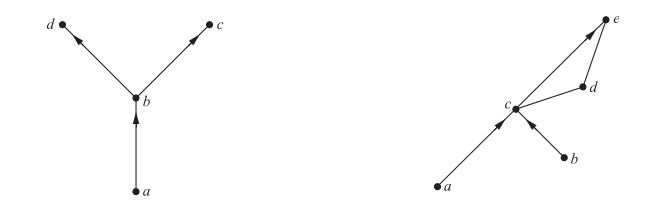
\includegraphics[max size={\textwidth}{\textheight}]{Semilatice_files/Semilatice_17_0.jpeg}
    \par
    \end{center}
    
            \end{InvisibleVerbatim}
            
        
    
In imaginea de mai sus, Fig 2(a), $S=\{a,b,c,d\}$ , multimea $S$ are
elementul minim, dar nu are maximum. In fig 2(b) $S=\{a,b,c,d, e\}$ ,
$S$ are maximum dar nu are minimum.

An ordered set $S$ having the property that each of its non-empty
subsets has a first element, is said to be \emph{\textbf{well ordered}}.\subsection{Operații Binare / Binary
Operatioins}\label{operaux21bii-binare-binary-operatioins}

Definitions:

\begin{itemize}
\itemsep1pt\parskip0pt\parsep0pt
\item
  A binary operation $\circ$ on a set $S$ is called \textbf{commutative}
  whenever $x \circ y = y \circ x$ for all $x, y \in S$
\item
  A binary operation $\circ$ on a set $S$ is called \textbf{associative}
  whenever $(x \circ y) \circ z = x \circ ( y \circ z)$ for all
  $x, y, z \in S$:
\end{itemize}\subsection{Quasi-order Relation}\label{quasi-order-relation}

Source:
\href{http://alas.matf.bg.ac.rs/~mi10103/predavanja/_ds1/DS.pdf}{Discrete
Mathematics by S Lipschutz and M Lipson}

Suppose ≺ is a relation on a set $S$ satisfying the following two
properties:

\begin{enumerate}
\def\labelenumi{\arabic{enumi}.}
\itemsep1pt\parskip0pt\parsep0pt
\item
  (Irreflexive) For any a ∈ A, we have a /≺ a.
\item
  (Transitive) If a ≺ b, and b ≺ c, then a ≺ c.
\end{enumerate}

\textbf{Then ≺ is called a quasi-order on S.}

There is a close relationship between partial orders and quasi-orders.
Specifically, if $\preceq$ is a partial order on a set $S$ and we define
a ≺ b to mean $a \preceq b$ but $a \neq b$, then ≺ is a quasi-order on
$S$. Conversely, if ≺ is a quasi-order on a set $S$ and we define
$a \preceq b$ to mean $a \prec b$ or a = b, then $\preceq$ is a partial
order on $S$.

    % Make sure that atleast 4 lines are below the HR
    \needspace{4\baselineskip}

    
        \vspace{6pt}
        \makebox[0.1\linewidth]{\smaller\hfill\tt\color{nbframe-in-prompt}In\hspace{4pt}{[}{]}:\hspace{4pt}}\\*
        \vspace{-2.65\baselineskip}
        \begin{ColorVerbatim}
            \vspace{-0.7\baselineskip}
            \begin{Verbatim}[commandchars=\\\{\}]

\end{Verbatim}

            
                \vspace{0.3\baselineskip}
            
        \end{ColorVerbatim}
    

        

        \renewcommand{\indexname}{Index}
        \printindex

    % End of document
    \end{document}


